\documentclass{standalone}

\usepackage{tikz}
\usepackage{tkz-euclide}
\usetikzlibrary{calc}
\usetikzlibrary{positioning}
\usetikzlibrary{arrows.meta}
\usetikzlibrary{shapes,snakes}

\usepackage{times}

\definecolor{myblue}{rgb}{0.0,0.5,0.8}

\begin{document}
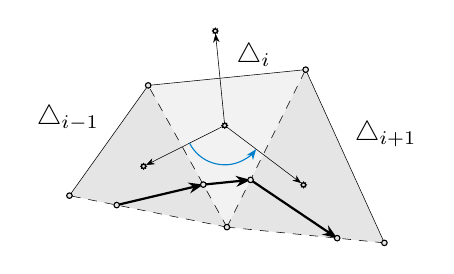
\begin{tikzpicture}[%
  >={Stealth[scale=0.8]},
  face/.style={star, star points = 8},
  scale=2.0,
]

  \tkzDefPoint(0.0, 0.0){v0}
  \tkzDefPoint(1.0, -0.1){v1}
  \tkzDefPoint(0.5, 1.0){v2}
  \tkzDefPoint(-0.5, 0.9){v3}
  \tkzDefPoint(-1.0, 0.2){v4}

  \tkzDefPointOnLine[pos=0.7](v0,v4)\tkzGetPoint{e0}
  \tkzDefPointOnLine[pos=0.3](v0,v3)\tkzGetPoint{e1}
  \tkzDefPointOnLine[pos=0.3](v0,v2)\tkzGetPoint{e2}
  \tkzDefPointOnLine[pos=0.7](v0,v1)\tkzGetPoint{e3}

  \tkzDefTriangleCenter[in](v0,v1,v2)\tkzGetPoint{fr}
  \tkzDefTriangleCenter[in](v0,v2,v3)\tkzGetPoint{f}
  \tkzDefTriangleCenter[in](v0,v3,v4)\tkzGetPoint{fl}
  \tkzDefPointBy[reflection=over v2--v3](f)\tkzGetPoint{fu}

  \tkzFillPolygon[color=black!10](v0,v1,v2)
  \tkzFillPolygon[color=black!5](v0,v2,v3)
  \tkzFillPolygon[color=black!10](v0,v3,v4)

  \tkzDrawSegments[dashed](v0,v1 v0,v2 v0,v3 v0,v4)
  \tkzDrawSegments(v1,v2 v2,v3 v3,v4)
  \tkzDrawPoints(v0,v1,v2,v3,v4)

  \tkzDrawSegments[->,add=0 and -0.03](f,fr f,fl f,fu)
  \tkzDrawArc[->,myblue,thin,R with nodes](f,0.25)(fl,fr)
  \tkzDrawPoints[star, star points = 8, scale = 1.0](fr,f,fl,fu)

  \tkzDrawSegments[thick,->](e0,e1 e1,e2 e2,e3)
  \tkzDrawPoints(e0,e1,e2,e3)

  \tkzLabelSegment[above right](v1,v2){$\triangle_{i+1}$}
  \tkzLabelSegment[above right](v2,v3){$\triangle_i$}
  \tkzLabelSegment[above left](v3,v4){$\triangle_{i-1}$}

\end{tikzpicture}
\end{document}
